\chapter{scanf()}
\index{\CStandardLibrary!scanf()}
\label{label_scanf}

\RU{Теперь попробуем использовать scanf().}\EN{Now let's use scanf().}

% sections
\section{\RU{Простой пример}\EN{Simple example}}

\lstinputlisting{patterns/04_scanf/1_simple/ex1.c}

\RU{Да, согласен, использовать \scanf в наши времена для того, чтобы спросить у пользователя что-то, 
не самая хорошая идея.
Но я хотел проиллюстрировать передачу указателя на переменную типа \Tint.}
\EN{OK, I agree, it is not clever to use \scanf for user interactions nowadays. 
I wanted, however, to illustrate passing a pointer to a variable of type \Tint.}

\subsection{\RU{Об указателях}\EN{About pointers}}
\index{\CLanguageElements!\Pointers}

\RU{Это одна из фундаментальных вещей в компьютерных науках.}\EN{Pointers are one of the fundamental concepts in computer science.}
\RU{Часто большой массив, структуру или объект передавать в другую функцию никак не выгодно, 
а передать её адрес куда проще.}
\EN{Often, passing a large array, structure or object as an argument to another function is too expensive, 
while passing their address is much cheaper.}
\RU{К тому же, если вызываемая функция (\gls{callee}) должна изменить что-то в этом большом массиве или структуре,
то возвращать её полностью\EMDASH{}это так же абсурдно.}
\EN{In addition if the \gls{callee} function needs to modify something in the large array or structure received as a parameter and return back the entire structure then the situation is close to absurd.}
\RU{Так что самое простое, что можно сделать, это передать в функцию-\gls{callee} адрес массива или структуры,
и пусть \gls{callee} что-то там изменит.}
\EN{So the simplest thing to do is to pass the address of the array or structure to the \gls{callee} function,
and let it change what needs to be changed.}

\RU{Указатель в}\EN{A pointer in} \CCpp \RU{\EMDASH{}это просто адрес какого-либо места в памяти.}
\EN{is simply an address of some memory location.}

\index{x86-64}
\RU{В x86 адрес представляется в виде 32-битного числа (т.е., занимает 4 байта), а в x86--64 как 64-битное число 
(занимает 8 байт).}
\EN{In x86, the address is represented as a 32-bit number (i.e., it is occupying 4 bytes), while in x86--64 it is a 64-bit number (occupying 8 bytes).}
\RU{Кстати, отсюда негодование некоторых людей, связанное с переходом на x86-64\EMDASH{}на этой архитектуре все указатели
занимают в 2 раза больше места, в том числе и в ``дорогой'' кэш-памяти.}
\EN{By the way, that is the reason behind some people's indignation related to switching to x86-64\EMDASH{}all pointers
in the x64-architecture require twice as much space, including cache memory, which is ``expensive'' place.}

\index{\CStandardLibrary!memcpy()}
\RU{При некотором упорстве можно работать только с безтиповыми указателями (\TT{void*})}\EN{
It is possible to work with untyped pointers only, given some effort}; \RU{например,}\EN{e.g.} 
\RU{стандартная функция Си}\EN{the standard C function} \TT{memcpy()},
\RU{копирующая блок из одного места памяти в другое}\EN{that copies a block from one memory location to another}, 
\RU{принимает на вход 2 указателя типа}\EN{takes 2 pointers of type } \TT{void*}\EN{ as arguments}, 
\RU{потому что нельзя
заранее предугадать, какого типа блок вы собираетесь копировать. 
Да в общем, тип данных не важен, важен только размер блока.}
\EN{since it is impossible to predict the type of the data you would like to copy. 
Data types are not important, only the block size matters.}

\RU{Также указатели широко используются, когда функции нужно вернуть более одного значения}
\EN{Pointers are also widely used when a function needs to return more than one value}
(\RU{мы еще вернемся к этому в будущем}\EN{we are going to get back to this later}
\ifx\LITE\undefined
~(\myref{label_pointers})
\fi
).
\IT{scanf()} \RU{\EMDASH{}это как раз такой случай}\EN{is such a case}. 
\RU{Помимо того, что этой функции нужно показать, сколько значений
было прочитано успешно, ей еще и нужно вернуть сами значения.}
\EN{Besides the fact that the function needs to indicate how many values were successfully read, 
it also needs to return all these values.}

\RU{Тип указателя в}\EN{In} \CCpp \RU{нужен для проверки типов на стадии компиляции.}
\EN{the pointer type is only needed for compile-time type checking.}
\RU{Внутри, в скомпилированном коде, никакой информации о типах указателей нет вообще.}
\EN{Internally, in the compiled code there is no information about pointer types at all.}

\subsection{x86}

\subsubsection{MSVC}

\RU{Что получаем на ассемблере компилируя MSVC 2010:}
\EN{Here is what we get after compiling with MSVC 2010:}

\lstinputlisting{patterns/04_scanf/1_simple/ex1_MSVC.asm.\LANG}

\RU{Переменная \TT{x} является локальной.}\EN{\TT{x} is a local variable.} 

\RU{По стандарту \CCpp она доступна только из этой же функции и ниоткуда более. 
Так получилось, что локальные переменные располагаются в стеке. 
Может быть, можно было бы использовать и другие варианты, но в x86 это традиционно так.}
\EN{According to the \CCpp standard it must be visible only in this function and not from any other external scope. 
Traditionally, local variables are stored on the stack. 
There are probably other ways to allocate them, but in x86 that is the way it is.}

\index{x86!\Instructions!PUSH}
\RU{Следующая после пролога инструкция \TT{PUSH ECX} не ставит своей целью сохранить 
значение регистра \ECX. 
(Заметьте отсутствие соответствующей инструкции \TT{POP ECX} в конце функции)}
\EN{The goal of the instruction following the function prologue, \TT{PUSH ECX}, is not to save the \ECX state 
(notice the absence of corresponding \TT{POP ECX} at the function's end).}

\RU{Она на самом деле выделяет в стеке 4 байта для хранения \TT{x} в будущем.} 
\EN{In fact it allocates 4 bytes on the stack for storing the \TT{x} variable.} 

\label{stack_frame}
\index{\Stack!\RU{Стековый фрейм}\EN{Stack frame}}
\index{x86!\Registers!EBP}
\RU{Доступ к \TT{x} будет осуществляться при помощи объявленного макроса \TT{\_x\$} 
(он равен -4) и регистра \EBP указывающего на текущий фрейм.}
\EN{\TT{x} will be accessed with the assistance of the \TT{\_x\$} macro 
(it equals to -4) and the \EBP register pointing to the current frame.}

\RU{Вообще, во все время исполнения функции, \EBP указывает на текущий \glslink{stack frame}{фрейм} и через \TT{EBP+смещение}
можно иметь доступ как к локальным переменным функции, так и аргументам функции.} 
\EN{Over the span of the function's execution, \EBP will be pointing to the current \gls{stack frame} making it possible to access local variables and function arguments via \TT{EBP+offset}.}

\index{x86!\Registers!ESP}
\RU{Можно было бы использовать \ESP, но он во время исполнения функции часто меняется, а это не удобно. 
Так что можно сказать, что \EBP это \IT{замороженное состояние} \ESP на момент начала исполнения функции.}
\EN{It is also possible to use \ESP for the same purpose, although that is not very convenient since it changes frequently.
The value of the \EBP could be perceived as a \IT{frozen state} of the value in \ESP at the start of the function's execution.}

% FIXME это уже было в 02_stack?
\RU{Разметка типичного стекового \glslink{stack frame}{фрейма} в 32-битной среде}
\EN{Here is a typical \gls{stack frame} layout in 32-bit environment}:

\begin{center}
\begin{tabular}{ | l | l | }
\hline
\dots & \dots \\
\hline
EBP-8 & \RU{локальная переменная}\EN{local variable} \#2, \MarkedInIDAAs{} \TT{var\_8} \\
\hline
EBP-4 & \RU{локальная переменная}\EN{local variable} \#1, \MarkedInIDAAs{} \TT{var\_4} \\
\hline
EBP & \RU{сохраненное значение}\EN{saved value of} \EBP \\
\hline
EBP+4 & \RU{адрес возврата}\EN{return address} \\
\hline
EBP+8 & \argument \#1, \MarkedInIDAAs{} \TT{arg\_0} \\
\hline
EBP+0xC & \argument \#2, \MarkedInIDAAs{} \TT{arg\_4} \\
\hline
EBP+0x10 & \argument \#3, \MarkedInIDAAs{} \TT{arg\_8} \\
\hline
\dots & \dots \\
\hline
\end{tabular}
\end{center}

\RU{У функции \scanf в нашем примере два аргумента.}\EN{The \scanf function in our example has two arguments.}

\RU{Первый ~--- указатель на строку, содержащую \TT{``\%d''} и второй ~--- адрес переменной \TT{x}.} 
\EN{The first one is a pointer to the string containing \TT{``\%d''} and the second is the address of the \TT{x} variable.} 

\index{x86!\Instructions!LEA}
\RU{Вначале адрес \TT{x} помещается в регистр \EAX при помощи инструкции \TT{lea eax, DWORD PTR \_x\$[ebp]}.}
\EN{First, the \TT{x} variable's address is loaded into the \EAX register by the \TT{lea eax, DWORD PTR \_x\$[ebp]} instruction}

\RU{Инструкция \LEA означает \IT{load effective address}, и часто используется для формирования адреса чего-либо}
\EN{\LEA stands for \IT{load effective address}, and is often used for forming an address}
~(\myref{sec:LEA}).

\RU{Можно сказать, что в данном случае \LEA просто помещает в \EAX результат суммы значения в регистре 
\EBP и макроса \TT{\_x\$}.}
\EN{We could say that in this case \LEA simply stores the sum of the \EBP register value and the \TT{\_x\$} macro in the \EAX register.}

\RU{Это тоже что и}\EN{This is the same as} \TT{lea eax, [ebp-4]}.

\RU{Итак, от значения \EBP отнимается $4$ и помещается в \EAX.
Далее значение \EAX заталкивается в стек и вызывается \scanf.}
\EN{So, $4$ is being subtracted from the \EBP register value and the result is loaded in the \EAX register.
Next the \EAX register value is pushed into the stack and \scanf is being called.}

\RU{После этого вызывается \printf. Первый аргумент вызова которого, строка:} 
\EN{\printf is being called after that with its first argument - a pointer to the string:} \TT{``You entered \%d...\textbackslash{}n''}.

\RU{Второй аргумент: \TT{mov ecx, [ebp-4]}, эта инструкция помещает в \ECX не адрес переменной \TT{x}, 
а его значение, что там сейчас находится.}
\EN{The second argument is prepared with: \TT{mov ecx, [ebp-4]}.
The instruction stores the \TT{x} variable value and not its address, in the \ECX register.}

\RU{Далее значение \ECX заталкивается в стек и вызывается последний \printf.}
\EN{Next the value in the \ECX is stored on the stack and the last \printf is being called.}

\ifdefined\IncludeOlly
\clearpage
\subsection{MSVC + \olly}
\index{\olly}

\RU{Попробуем этот же пример в}\EN{Let's try this example in} \olly.
\RU{Загружаем, нажимаем F8 (\stepover) до тех пор, пока не окажемся в своем исполняемом файле,
а не в}\EN{Let's load it and keep pressing F8 (\stepover) until we reach our executable file
instead of} \TT{ntdll.dll}.
\RU{Прокручиваем вверх до тех пор, пока не найдем \main}\EN{Scroll up until \main appears}.
\RU{Щелкаем на первой инструкции (\TT{PUSH EBP}), нажимаем F2 (\IT{set a breakpoint}), 
затем F9 (\IT{Run}) и точка останова срабатывает на начале \main.}
\EN{Click on the first instruction (\TT{PUSH EBP}), press F2 (\IT{set a breakpoint}), 
then F9 (\IT{Run}).
The breakpoint will be triggered when \main begins.}

\RU{Трассируем до того места, где готовится адрес переменной $x$}%
\EN{Let's trace to the point where the address of the variable $x$ is calculated}:

\begin{figure}[H]
\centering
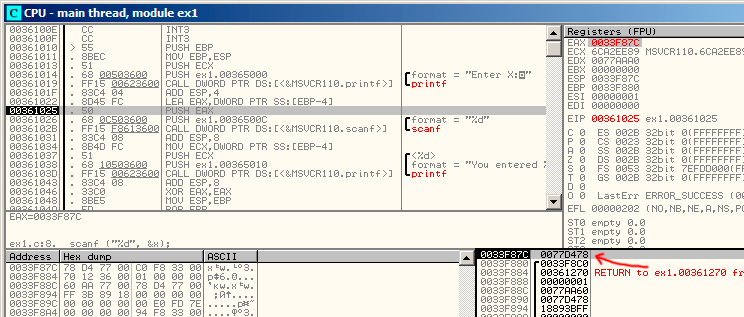
\includegraphics[scale=\FigScale]{patterns/04_scanf/1_simple/ex1_olly_1.png}
\caption{\olly: \RU{вычисляется адрес локальной переменной}\EN{The address of the local variable is calculated}}
\label{fig:scanf_ex1_olly_1}
\end{figure}

\RU{На \EAX в окне регистров можно нажать правой кнопкой и далее выбрать}
\EN{Right-click the \EAX in the registers window and then select} \q{Follow in stack}.
\RU{Этот адрес покажется в окне стека.}
\EN{This address will appear in the stack window.}
\RU{Смотрите, это переменная в локальном стеке. Я нарисовал там красную стрелку}\EN{The red arrow, I have added, points to the variable in the local stack}.
\RU{И там сейчас какой-то мусор}\EN{At that moment this location contains some garbage} (\TT{0x6E494714}).
\RU{Адрес этого элемента стека сейчас, при помощи \PUSH запишется в этот же стек рядом}%
\EN{Now with the help of \PUSH instruction the address of this stack element is going to be stored to the same stack on the next position}.
\RU{Трассируем при помощи F8 вплоть до конца исполнения \scanf}\EN{Let's trace with F8 until the \scanf execution completes}.
\RU{А пока \scanf исполняется, в консольном окне, вводим, например, 123}%
\EN{During the \scanf execution, we input, for example, 123, in the console window}:

\begin{figure}[H]
\centering
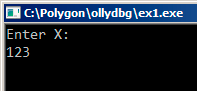
\includegraphics[scale=\NormalScale]{patterns/04_scanf/1_simple/ex1_olly_2.png}
\caption{\RU{Ввод пользователя в консольном окне}\EN{User input in the console window}}
\label{fig:scanf_ex1_olly_2}
\end{figure}

\clearpage
\RU{Вот тут }\scanf \RU{отработал}\EN{completed its execution already}:

\begin{figure}[H]
\centering
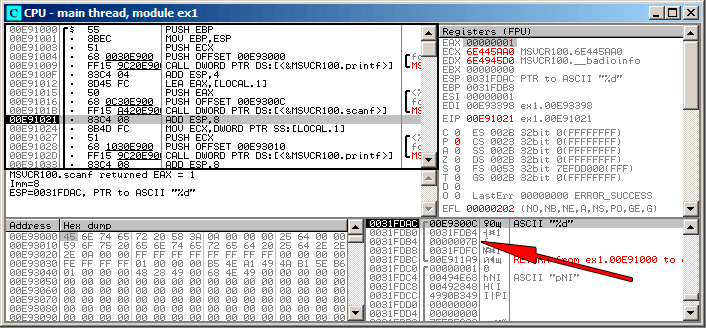
\includegraphics[scale=\FigScale]{patterns/04_scanf/1_simple/ex1_olly_3.png}
\caption{\olly: \scanf \RU{исполнилась}\EN{executed}}
\label{fig:scanf_ex1_olly_3}
\end{figure}

\scanf \RU{вернул}\EN{returns} $1$ \InENRU \EAX, \RU{что означает, что он успешно прочитал одно 
значение}\EN{which implies that it has read successfully one value}.
\RU{В наблюдаемом нами элементе стека теперь}\EN{If we look again at the stack element corresponding to the local variable it now contains} \TT{0x7B} (123).

\clearpage
\RU{Чуть позже это значение копируется из стека в регистр \ECX и передается в \printf}
\EN{Later this value is copied from the stack to the \ECX register and passed to \printf}:

\begin{figure}[H]
\centering
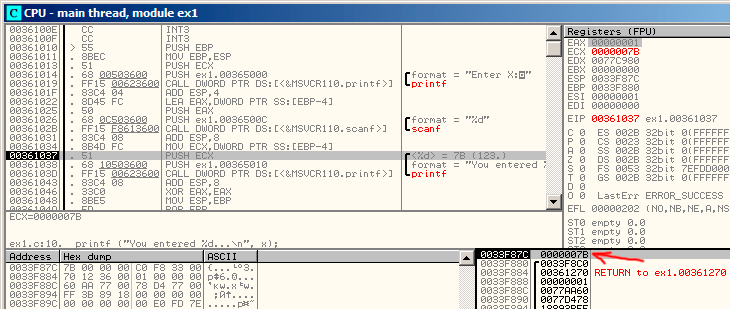
\includegraphics[scale=\FigScale]{patterns/04_scanf/1_simple/ex1_olly_4.png}
\caption{\olly: \RU{готовим значение для передачи в}\EN{preparing the value for passing to} \printf}
\label{fig:scanf_ex1_olly_4}
\end{figure}

\fi

\subsubsection{GCC}

\RU{Попробуем тоже самое скомпилировать в Linux при помощи GCC 4.4.1:}
\EN{Let's try to compile this code in GCC 4.4.1 under Linux:}

\lstinputlisting{patterns/04_scanf/1_simple/ex1_GCC.asm}

\index{puts() \RU{вместо}\EN{instead of} printf()}
\RU{GCC заменил первый вызов \printf на \puts, почему это было сделано, 
уже было описано раннее~(\myref{puts}).}
\EN{GCC replaced the \printf call with call to \puts. The reason for this was explained in ~(\myref{puts}).}

% TODO: rewrite
%\RU{Почему \scanf переименовали в \TT{\_\_\_isoc99\_scanf}, я честно говоря, пока не знаю.}
%\EN{Why \scanf is renamed to \TT{\_\_\_isoc99\_scanf}, I do not know yet.}
% 
% Apparently it has to do with the ISO c99 standard compliance. By default GCC allows specifying a standard to adhere to.
% For example if you compile with -std=c89 the outputted assmebly file will contain scanf and not __isoc99__scanf. I guess current GCC version adhares to c99 by default.
% According to my understanding the two implementations differ in the set of suported modifyers (See printf man page)


\RU{Далее все как и прежде ~--- параметры заталкиваются через стек при помощи \MOV.}
\EN{As in the MSVC example ~---the arguments are placed on the stack using the \MOV instruction.}
\subsection{x64}

\index{x86-64}
\RU{Всё то же самое, только используются регистры вместо стека для передачи аргументов функций.}%
\EN{The picture here is similar with the difference that the registers, rather than the stack, are used for arguments passing.}%
\PTBR{A situação aqui é parecida, mas com a diferença de que os registradores, ao invés da pilha, são usados para passar argumentos.}%

\subsubsection{MSVC}

\lstinputlisting[caption=MSVC 2012 x64]{patterns/04_scanf/1_simple/ex1_MSVC_x64.asm.\LANG}

\ifdefined\IncludeGCC
\subsubsection{GCC}

\lstinputlisting[caption=\Optimizing GCC 4.4.6 x64]{patterns/04_scanf/1_simple/ex1_GCC_x64.s.\LANG}
\fi


\ifdefined\IncludeARM
\subsection{ARM}

\subsubsection{\OptimizingKeilVI (\ThumbMode)}

\begin{lstlisting}
.text:00000042             scanf_main
.text:00000042
.text:00000042             var_8           = -8
.text:00000042
.text:00000042 08 B5                       PUSH    {R3,LR}
.text:00000044 A9 A0                       ADR     R0, aEnterX     ; "Enter X:\n"
.text:00000046 06 F0 D3 F8                 BL      __2printf
.text:0000004A 69 46                       MOV     R1, SP
.text:0000004C AA A0                       ADR     R0, aD          ; "%d"
.text:0000004E 06 F0 CD F8                 BL      __0scanf
.text:00000052 00 99                       LDR     R1, [SP,#8+var_8]
.text:00000054 A9 A0                       ADR     R0, aYouEnteredD___ ; "You entered %d...\n"
.text:00000056 06 F0 CB F8                 BL      __2printf
.text:0000005A 00 20                       MOVS    R0, #0
.text:0000005C 08 BD                       POP     {R3,PC}
\end{lstlisting}

\index{\CLanguageElements!\Pointers}
\RU{Чтобы \scanf мог вернуть значение, ему нужно передать указатель на переменную типа \Tint.}
\EN{In order for \scanf to be able to read item it needs a parameter---pointer to an \Tint.}
\Tint\RU{~--- 32-битное значение, для его хранения нужно только 4 байта, и оно помещается в 
32-битный регистр.}
\EN{is 32-bit, so we need 4 bytes to store it somewhere in memory, and it fits exactly 
in a 32-bit register.}
\index{IDA!var\_?}
\RU{Место для локальной переменной \TT{x} выделяется в стеке, \IDA наименовала её \IT{var\_8}. 
Впрочем, место для неё выделять не обязательно, т.к. \glslink{stack pointer}{указатель стека} \ac{SP} уже указывает на место, 
свободное для использования.}\EN{A place for the local variable \TT{x} is allocated in the stack and \IDA
has named it \IT{var\_8}. It is not necessary, however, to allocate a such since \ac{SP} (\gls{stack pointer}) is already pointing to that space and it can be used directly.}
\RU{Так что значение указателя \ac{SP} копируется в регистр \Reg{1}, и вместе с format-строкой, 
передается в \scanf.}
\EN{So, \ac{SP}'s value is copied to the \Reg{1} register and, together with the format-string, passed
to \scanf.}
\index{ARM!\Instructions!LDR}
\RU{Позже, при помощи инструкции \TT{LDR}, это значение перемещается из стека в регистр \Reg{1}, 
чтобы быть переданным в \printf.}\EN{Later, with the help of the \TT{LDR} instruction, this value is moved
from the stack to the \Reg{1} register in order to be passed to \printf.}

\subsubsection{ARM64}

\lstinputlisting[caption=\NonOptimizing GCC 4.9.1 ARM64,numbers=left]{patterns/04_scanf/1_simple/ARM64_GCC491_O0.s.\LANG}

\RU{Под стековый фрейм выделяется 32 байта, что больше чем нужно. Вероятно, это связано с выравниваем по границе памяти?}%
\EN{There is 32 bytes are allocated for stack frame, which is bigger than it needed. Perhaps, some memory aligning issue?}
\RU{Самая интересная часть~--- это поиск места под переменную $x$ в стековом фрейме (строка 22).}
\EN{The most interesting part is finding space for the $x$ variable in the stack frame (line 22).}
\RU{Почему 28? Почему-то, компилятор решил расположить эту переменную в конце стекового фрейма, а не в начале.}%
\EN{Why 28? Somehow, compiler decided to place this variable at the end of stack frame instead of beginning.}
\RU{Адрес потом передается в \scanf, которая просто сохраняет значение, введенное пользователем, в памяти
по этому адресу.}
\EN{The address is passed to \scanf, which just stores the user input value in the memory at that address.}
\RU{Это 32-битное значение типа \Tint}\EN{This is 32-bit value of type \Tint}.
\RU{Значение загружается в строке 27 и затем передается в \printf.}
\EN{The value is fetched at line 27 and then passed to \printf.}


\fi
\ifdefined\IncludeMIPS
\subsection{MIPS}

\RU{Для переменной $x$ выделено место в стеке, и к нему будут производиться обращения как $\$sp+24$.}
\EN{A place in the local stack is allocated for the $x$ variable, and it is to be referred as $\$sp+24$.}
\myindex{MIPS!\Instructions!LW}
\RU{Её адрес передается в \scanf, а значение прочитанное от пользователя загружается используя 
инструкцию LW (\q{Load Word}~--- загрузить слово) и затем оно передается в \printf.}
\EN{Its address is passed to \scanf, and the user input values is loaded using the LW (\q{Load Word}) instruction
and then passed to \printf.}

\lstinputlisting[caption=\Optimizing GCC 4.4.5 (\assemblyOutput)]{patterns/04_scanf/1_simple/MIPS/ex1.O3.s.\LANG}

\RU{IDA показывает разметку стека следующим образом:}
\EN{IDA displays the stack layout as follows:}

\lstinputlisting[caption=\Optimizing GCC 4.4.5 (IDA)]{patterns/04_scanf/1_simple/MIPS/ex1.O3.IDA.lst.\LANG}

% TODO non-optimized version?

\fi

\ifdefined\ENGLISH
\newcommand{\GlobalVarsSectionName}{Global variables}
\section{\GlobalVarsSectionName}
\myindex{\GlobalVarsSectionName}
\label{scanf_global_variable}

What if the \TT{x} variable from the previous example was not local but a global one? 
Then it would have been accessible from any point, not only from the function body. 
Global variables are considered \gls{anti-pattern}, but for the sake of the experiment, we could do this.

\lstinputlisting{patterns/04_scanf/2_global/ex2_EN.c}
\fi

\ifdefined\RUSSIAN
\newcommand{\GlobalVarsSectionName}{Глобальные переменные}
\section{\GlobalVarsSectionName}
\myindex{\GlobalVarsSectionName}
\label{scanf_global_variable}

А что если переменная \TT{x} из предыдущего примера будет глобальной переменной, а не локальной? 
Тогда к ней смогут обращаться из любого другого места, а не только из тела функции. 
Глобальные переменные считаются \glslink{anti-pattern}{анти-паттерном},
но ради примера мы можем себе это позволить.

\lstinputlisting{patterns/04_scanf/2_global/ex2_RU.c}
\fi

\ifdefined\BRAZILIAN
\newcommand{\GlobalVarsSectionName}{Variáveis globais}
\section{\GlobalVarsSectionName}
\myindex{\GlobalVarsSectionName}
\label{scanf_global_variable}

E se a variável \TT{x} do último exemplo não fosse local, mas sim global?
Então ela teria que ser acessível de qualquer ponto, não somente pelo corpo da função.
Variáveis globais são consideradas maus hábitos, mas pelo bem do experimento, nós faremos isso.

% TODO translate
\lstinputlisting{patterns/04_scanf/2_global/ex2_EN.c}
\fi


\EN{\subsectionold{MSVC: x86}

\lstinputlisting{patterns/04_scanf/2_global/ex2_MSVC.asm}

In this case the \TT{x} variable is defined in the \TT{\_DATA} segment and no memory is allocated in the local stack. It is accessed directly, not through the stack. 
Uninitialized global variables take no space in the executable file
(indeed, why one needs to allocate space for variables initially set to zero?), 
but when someone accesses their address, 
the \ac{OS} will allocate a block of zeroes there\footnote{That is how a \ac{VM} behaves}.

Now let's explicitly assign a value to the variable:

\lstinputlisting{patterns/04_scanf/2_global/default_value_EN.c}

We got:

\begin{lstlisting}
_DATA	SEGMENT
_x	DD	0aH

...
\end{lstlisting}

Here we see a value \TT{0xA} of DWORD type (DD stands for DWORD = 32 bit) for this variable.

If you open the compiled .exe in \IDA, you can see the \IT{x} variable placed at the beginning of 
the \TT{\_DATA} segment, and after it you can see text strings.

If you open the compiled .exe from the previous example in \IDA, where the value of \IT{x} was not set, you would see something like this:

\begin{lstlisting}
.data:0040FA80 _x              dd ?                    ; DATA XREF: _main+10
.data:0040FA80                                         ; _main+22
.data:0040FA84 dword_40FA84    dd ?                    ; DATA XREF: _memset+1E
.data:0040FA84                                         ; unknown_libname_1+28
.data:0040FA88 dword_40FA88    dd ?                    ; DATA XREF: ___sbh_find_block+5
.data:0040FA88                                         ; ___sbh_free_block+2BC
.data:0040FA8C ; LPVOID lpMem
.data:0040FA8C lpMem           dd ?                    ; DATA XREF: ___sbh_find_block+B
.data:0040FA8C                                         ; ___sbh_free_block+2CA
.data:0040FA90 dword_40FA90    dd ?                    ; DATA XREF: _V6_HeapAlloc+13
.data:0040FA90                                         ; __calloc_impl+72
.data:0040FA94 dword_40FA94    dd ?                    ; DATA XREF: ___sbh_free_block+2FE
\end{lstlisting}

\TT{\_x} is marked with \TT{?} with the rest of the variables that do not need to be initialized. 
This implies that after loading the .exe to the memory, a space for all these variables is to be 
allocated and filled with zeroes [\CNineNineStd 6.7.8p10].
But in the .exe file these uninitialized variables do not occupy anything.
This is convenient for large arrays, for example.

\EN{\input{patterns/04_scanf/2_global/olly_EN}}
\RU{\input{patterns/04_scanf/2_global/olly_RU}}
\ITA{\input{patterns/04_scanf/2_global/olly_ITA}}


\subsectionold{GCC: x86}

\myindex{ELF}
The picture in Linux is near the same, with the difference that the uninitialized variables are located in the \TT{\_bss} segment. 
In \ac{ELF} file this segment has the following attributes:

\begin{lstlisting}
; Segment type: Uninitialized
; Segment permissions: Read/Write
\end{lstlisting}

If you, however, initialise the variable with some value e.g. 10, 
it is to be placed in the \TT{\_data} segment, which has the following attributes:

\begin{lstlisting}
; Segment type: Pure data
; Segment permissions: Read/Write
\end{lstlisting}

\subsectionold{MSVC: x64}

\lstinputlisting[caption=MSVC 2012 x64]{patterns/04_scanf/2_global/ex2_MSVC_x64_EN.asm}

The code is almost the same as in x86.
Please note that the address of the $x$ variable is passed to \TT{scanf()} using a \LEA instruction,
while the variable's value is passed to the second \printf using a \MOV instruction.
\TT{DWORD PTR}---is a part of the assembly language (no relation to the machine code),
indicating that the variable data size is 32-bit and the \MOV instruction has to be encoded accordingly.

}
\RU{\subsubsection{MSVC: x86}

\lstinputlisting{patterns/04_scanf/2_global/ex2_MSVC.asm}

В целом ничего особенного. Теперь \TT{x} объявлена в сегменте \TT{\_DATA}. 
Память для неё в стеке более не выделяется.
Все обращения к ней происходит не через стек, а уже напрямую. 
Неинициализированные глобальные переменные не занимают места в исполняемом файле
(и действительно, зачем в исполняемом файле
нужно выделять место под изначально нулевые переменные?), но тогда, когда к этому месту в памяти
кто-то обратится, \ac{OS} подставит туда блок, состоящий из нулей\footnote{Так работает \ac{VM}}.

Попробуем изменить объявление этой переменной:

\lstinputlisting{patterns/04_scanf/2_global/default_value_RU.c}

Выйдет в итоге:

\begin{lstlisting}
_DATA	SEGMENT
_x	DD	0aH

...
\end{lstlisting}

Здесь уже по месту этой переменной записано \TT{0xA} с типом DD (dword = 32 бита).

Если вы откроете скомпилированный .exe-файл в \IDA, то увидите, что \IT{x} 
находится в начале сегмента \TT{\_DATA}, после этой переменной будут текстовые строки.

А вот если вы откроете в \IDA .exe скомпилированный в прошлом примере, где значение \IT{x} не определено, то вы увидите:

\begin{lstlisting}
.data:0040FA80 _x              dd ?                    ; DATA XREF: _main+10
.data:0040FA80                                         ; _main+22
.data:0040FA84 dword_40FA84    dd ?                    ; DATA XREF: _memset+1E
.data:0040FA84                                         ; unknown_libname_1+28
.data:0040FA88 dword_40FA88    dd ?                    ; DATA XREF: ___sbh_find_block+5
.data:0040FA88                                         ; ___sbh_free_block+2BC
.data:0040FA8C ; LPVOID lpMem
.data:0040FA8C lpMem           dd ?                    ; DATA XREF: ___sbh_find_block+B
.data:0040FA8C                                         ; ___sbh_free_block+2CA
.data:0040FA90 dword_40FA90    dd ?                    ; DATA XREF: _V6_HeapAlloc+13
.data:0040FA90                                         ; __calloc_impl+72
.data:0040FA94 dword_40FA94    dd ?                    ; DATA XREF: ___sbh_free_block+2FE
\end{lstlisting}

\TT{\_x} обозначен как \TT{?}, наряду с другими переменными не требующими инициализации. 
Это означает, что при загрузке .exe в память, место под всё это выделено будет и будет заполнено
нулевыми байтами [\CNineNineStd 6.7.8p10]. 
Но в самом .exe ничего этого нет. Неинициализированные переменные не занимают места в исполняемых файлах. 
Это удобно для больших массивов, например.

\EN{\input{patterns/04_scanf/2_global/olly_EN}}
\RU{\input{patterns/04_scanf/2_global/olly_RU}}
\ITA{\input{patterns/04_scanf/2_global/olly_ITA}}


\subsubsection{GCC: x86}

\myindex{ELF}
В Linux всё почти также. За исключением того, что если значение \TT{x} не определено, 
то эта переменная будет находится в сегменте \TT{\_bss}.
В \ac{ELF} этот сегмент имеет такие атрибуты:

\begin{lstlisting}
; Segment type: Uninitialized
; Segment permissions: Read/Write
\end{lstlisting}

Ну а если сделать статическое присвоение этой переменной какого-либо
значения, например, 10, то она будет находится 
в сегменте \TT{\_data},
это сегмент с такими атрибутами:

\begin{lstlisting}
; Segment type: Pure data
; Segment permissions: Read/Write
\end{lstlisting}

\subsubsection{MSVC: x64}

\lstinputlisting[caption=MSVC 2012 x64]{patterns/04_scanf/2_global/ex2_MSVC_x64_RU.asm}

Почти такой же код как и в x86.
Обратите внимание что для \TT{scanf()} адрес переменной $x$ передается
при помощи инструкции \LEA, а во второй \printf передается само значение переменной при помощи \MOV.
\TT{DWORD PTR} --- это часть языка ассемблера (не имеющая отношения к машинным кодам) показывающая, что тип переменной в памяти именно 32-битный, 
и инструкция \MOV должна быть здесь закодирована соответственно.

}
\PTBR{\subsection{MSVC: x86}

\lstinputlisting{patterns/04_scanf/2_global/ex2_MSVC.asm}

Nesse caso, a variável \TT{x} é definida no segmento \TT{\_DATA} e nenhuma memória é alocada na pilha local.
Ela é acessada diretamente, não através da pilha.
Variáveis globais não inicialiadas não ocupam espaço no arquivo executável 
(realmente, ninguém precisa alocar espaço para uma variável inicialmente valendo zero), 
mas quando alguém acessa o endereço delas, o sistema operacional vai alocar um bloco contendo somente zeros nele.
\footnote{\ac{TBT}: That is how a \ac{VM} behaves}.

Agora vamos definir um valor para a variável:

% TODO translate
\lstinputlisting{patterns/04_scanf/2_global/default_value_EN.c}

Nós temos:

\begin{lstlisting}
_DATA	SEGMENT
_x	DD	0aH

...
\end{lstlisting}

Aqui nós vemos um valor \TT{0xA} do tipo DWORD (DD significa DWORD = 32 bits) para essa variável.

Se você abrir o .exe compilado no \IDA, você pode ver a variável \IT{x} colocada no começo do segmento \TT{\_DATA},
e depois disso você pode ver as strings.

Se você abrir o .exe compilado no exemplo anterior no \IDA, onde o valor de x não foi declarado, você poderá ver algo assim:

\begin{lstlisting}
.data:0040FA80 _x              dd ?                    ; DATA XREF: _main+10
.data:0040FA80                                         ; _main+22
.data:0040FA84 dword_40FA84    dd ?                    ; DATA XREF: _memset+1E
.data:0040FA84                                         ; unknown_libname_1+28
.data:0040FA88 dword_40FA88    dd ?                    ; DATA XREF: ___sbh_find_block+5
.data:0040FA88                                         ; ___sbh_free_block+2BC
.data:0040FA8C ; LPVOID lpMem
.data:0040FA8C lpMem           dd ?                    ; DATA XREF: ___sbh_find_block+B
.data:0040FA8C                                         ; ___sbh_free_block+2CA
.data:0040FA90 dword_40FA90    dd ?                    ; DATA XREF: _V6_HeapAlloc+13
.data:0040FA90                                         ; __calloc_impl+72
.data:0040FA94 dword_40FA94    dd ?                    ; DATA XREF: ___sbh_free_block+2FE
\end{lstlisting}

\TT{\_x} está marcada com \TT{?} juntamente com o resto das variáveis que não precisam ser inicializadas.
Isso implica que após carregar o .exe para a memória, um espaço para todas essas variáveis será alocado e preenchido com zeros [\CNineNineStd 6.7.8p10].
Mas no arquivo .exe essas variáveis não inicializadas não ocupam nenhum espaço.
Isso é conveniente para arrays grandes, por exemplo.

\EN{\input{patterns/04_scanf/2_global/olly_EN}}
\RU{\input{patterns/04_scanf/2_global/olly_RU}}
\ITA{\input{patterns/04_scanf/2_global/olly_ITA}}


\subsection{GCC: x86}

\PTBRph{}

\subsection{MSVC: x64}

% TODO translate
\lstinputlisting[caption=MSVC 2012 x64]{patterns/04_scanf/2_global/ex2_MSVC_x64_EN.asm}

O código é quase o mesmo que no x86.
Por favor, perceba que o endereço da variável x é passado para \TT{scanf()} usando uma instrução \LEA,
enquanto os valores das variáveis são passadas para o segundo \printf usando uma instrução \MOV.
\TT{DWORD PTR} é uma parte da linguagem assembly (sem relação com o código de máquina),
indicando que o tamanho da informação da variável é de 32-bits e que a instrução \MOV tem de ser codificada de acordo.

}
\ifdefined\IncludeARM
\EN{\subsection{ARM: \OptimizingKeilVI (\ThumbMode)}

\begin{lstlisting}
.text:00000000 ; Segment type: Pure code
.text:00000000                 AREA .text, CODE
...
.text:00000000 main
.text:00000000                 PUSH    {R4,LR}
.text:00000002                 ADR     R0, aEnterX     ; "Enter X:\n"
.text:00000004                 BL      __2printf
.text:00000008                 LDR     R1, =x
.text:0000000A                 ADR     R0, aD          ; "%d"
.text:0000000C                 BL      __0scanf
.text:00000010                 LDR     R0, =x
.text:00000012                 LDR     R1, [R0]
.text:00000014                 ADR     R0, aYouEnteredD___ ; "You entered %d...\n"
.text:00000016                 BL      __2printf
.text:0000001A                 MOVS    R0, #0
.text:0000001C                 POP     {R4,PC}
...
.text:00000020 aEnterX         DCB "Enter X:",0xA,0    ; DATA XREF: main+2
.text:0000002A                 DCB    0
.text:0000002B                 DCB    0
.text:0000002C off_2C          DCD x                   ; DATA XREF: main+8
.text:0000002C                                         ; main+10
.text:00000030 aD              DCB "%d",0              ; DATA XREF: main+A
.text:00000033                 DCB    0
.text:00000034 aYouEnteredD___ DCB "You entered %d...",0xA,0 ; DATA XREF: main+14
.text:00000047                 DCB 0
.text:00000047 ; .text         ends
.text:00000047
...
.data:00000048 ; Segment type: Pure data
.data:00000048                 AREA .data, DATA
.data:00000048                 ; ORG 0x48
.data:00000048                 EXPORT x
.data:00000048 x               DCD 0xA                 ; DATA XREF: main+8
.data:00000048                                         ; main+10
.data:00000048 ; .data         ends
\end{lstlisting}

So, the \TT{x} variable is now global and for this reason located in another segment, namely the data segment (\IT{.data}).
One could ask, why are the text strings located in the code segment (\IT{.text}) and \TT{x} is located right here?
Because it is a variable and by definition its value could change. Moreover it could possibly change often.
While text strings has constant type, they will not be changed, so they are located in the \IT{.text} segment.
\myindex{\RAM}
\myindex{\ROM}

The code segment might sometimes be located in a \ac{ROM} chip (remember, we now deal
with embedded microelectronics, and memory scarcity is common here), and changeable 
variables~---in \ac{RAM}.

It is not very economical to store constant variables in RAM when you have ROM.

Furthermore, constant variables in RAM must be initialized, because after powering on, the RAM, obviously, contains random information.

\myindex{Linker}

Moving forward, we see a pointer to the \TT{x} (\TT{off\_2C}) variable in the code segment, and that all
operations with the variable occur via this pointer.

That is because the \TT{x} variable could be located somewhere far from this particular code fragment, so its address
must be saved somewhere in close proximity to the code.
\myindex{ARM!\Instructions!LDR}

The \INS{LDR} instruction in Thumb mode can only address variables in a range of 1020 bytes from its location, 

and in in ARM-mode~---variables in range of $\pm{}4095$ bytes.

And so the address of the \TT{x} variable
must be located somewhere in close proximity, because there is no guarantee that the linker would be able to accommodate the variable somewhere nearby the code, it may well be even in an external memory chip!

\myindex{\CLanguageElements!const}
\myindex{\ROM}

One more thing: if a variable is declared as \IT{const}, the Keil compiler allocates it in 
the \TT{.constdata} segment.

Perhaps thereafter, the linker could place this segment in ROM too, along with the code segment.

\subsection{ARM64}

\lstinputlisting[caption=\NonOptimizing GCC 4.9.1 ARM64,numbers=left]{patterns/04_scanf/2_global/ARM64_GCC491_O0.s.\LANG}

\myindex{ARM!\Instructions!ADRP/ADD pair}

In this case the $x$ variable is declared as global and its address is calculated using 
the \INS{ADRP}/\INS{ADD} instruction pair (lines 21 and 25).

}
\RU{\subsection{ARM: \OptimizingKeilVI (\ThumbMode)}

\begin{lstlisting}
.text:00000000 ; Segment type: Pure code
.text:00000000                 AREA .text, CODE
...
.text:00000000 main
.text:00000000                 PUSH    {R4,LR}
.text:00000002                 ADR     R0, aEnterX     ; "Enter X:\n"
.text:00000004                 BL      __2printf
.text:00000008                 LDR     R1, =x
.text:0000000A                 ADR     R0, aD          ; "%d"
.text:0000000C                 BL      __0scanf
.text:00000010                 LDR     R0, =x
.text:00000012                 LDR     R1, [R0]
.text:00000014                 ADR     R0, aYouEnteredD___ ; "You entered %d...\n"
.text:00000016                 BL      __2printf
.text:0000001A                 MOVS    R0, #0
.text:0000001C                 POP     {R4,PC}
...
.text:00000020 aEnterX         DCB "Enter X:",0xA,0    ; DATA XREF: main+2
.text:0000002A                 DCB    0
.text:0000002B                 DCB    0
.text:0000002C off_2C          DCD x                   ; DATA XREF: main+8
.text:0000002C                                         ; main+10
.text:00000030 aD              DCB "%d",0              ; DATA XREF: main+A
.text:00000033                 DCB    0
.text:00000034 aYouEnteredD___ DCB "You entered %d...",0xA,0 ; DATA XREF: main+14
.text:00000047                 DCB 0
.text:00000047 ; .text         ends
.text:00000047
...
.data:00000048 ; Segment type: Pure data
.data:00000048                 AREA .data, DATA
.data:00000048                 ; ORG 0x48
.data:00000048                 EXPORT x
.data:00000048 x               DCD 0xA                 ; DATA XREF: main+8
.data:00000048                                         ; main+10
.data:00000048 ; .data         ends
\end{lstlisting}

Итак, переменная \TT{x} теперь глобальная, и она расположена, почему-то, в другом сегменте, а именно сегменте данных (\IT{.data}).
Можно спросить, почему текстовые строки расположены в сегменте кода (\IT{.text}), а \TT{x} нельзя было разместить тут же?

Потому что эта переменная, и как следует из определения, она может меняться. И может быть, меняться часто.

Ну а текстовые строки имеют тип констант, они не будут меняться, поэтому они располагаются в сегменте \IT{.text}.

\myindex{\RAM}
\myindex{\ROM}
Сегмент кода иногда может быть расположен в ПЗУ микроконтроллера (не забывайте, 
мы сейчас имеем дело с embedded-микроэлектроникой, где дефицит памяти~--- обычное дело),
а изменяемые переменные~--- в ОЗУ.

Хранить в ОЗУ неизменяемые данные, когда в наличии есть ПЗУ, не экономно.

К тому же, сегмент данных в ОЗУ с константами нужно инициализировать перед работой,
ведь, после включения ОЗУ, очевидно, она содержит в себе случайную информацию.

\myindex{Компоновщик}
Далее мы видим в сегменте кода хранится указатель на переменную \TT{x} (\TT{off\_2C}) и 
все операции с переменной происходят через этот указатель.

Это связано с тем, что переменная \TT{x} может быть расположена где-то довольно далеко от 
данного участка кода, так что её адрес нужно сохранить в непосредственной близости к этому коду.

\myindex{ARM!\Instructions!LDR}
Инструкция \INS{LDR} в Thumb-режиме может адресовать только переменные в пределах вплоть до 1020 байт от своего местоположения.

Эта же инструкция в ARM-режиме~--- переменные в пределах $\pm{}4095$ байт.

Таким образом,
адрес глобальной переменной \TT{x} нужно расположить в непосредственной близости, ведь нет никакой гарантии, 
что компоновщик\footnote{linker в англоязычной литературе} сможет разместить саму переменную где-то рядом, 
она может быть даже в другом чипе памяти!

\myindex{\CLanguageElements!const}
\myindex{\ROM}
Ещё одна вещь: если переменную объявить как \IT{const}, то компилятор Keil разместит её в сегменте \TT{.constdata}.

Должно быть, впоследствии компоновщик и этот сегмент сможет разместить в ПЗУ вместе с сегментом кода.

\subsection{ARM64}

\lstinputlisting[caption=\NonOptimizing GCC 4.9.1 ARM64,numbers=left]{patterns/04_scanf/2_global/ARM64_GCC491_O0.s.\LANG}

\myindex{ARM!\Instructions!ADRP/ADD pair}
Теперь $x$ это глобальная переменная, и её адрес вычисляется при помощи пары инструкций \INS{ADRP}/\INS{ADD} (строки 21 и 25).

}
\fi
\ifdefined\IncludeMIPS
\EN{\subsection{MIPS}

\subsubsection{Uninitialized global variable}

So now the $x$ variable is global.
Let's compile to executable file rather than object file and load it into \IDA.
IDA displays the $x$ variable in the .sbss ELF section (remember the \q{Global Pointer}? \myref{MIPS_GP}),
since the variable is not initialized at the start.

\lstinputlisting[caption=\Optimizing GCC 4.4.5 (IDA)]{patterns/04_scanf/2_global/MIPS/O3_IDA.lst.\LANG}

IDA reduces the amount of information, so we'll also do a listing using objdump and comment it:

\lstinputlisting[caption=\Optimizing GCC 4.4.5 (objdump),numbers=left]{patterns/04_scanf/2_global/MIPS/O3_objdump.txt.\LANG}

Now we see the $x$ variable address is read from a 64KiB data buffer using GP and adding negative offset to it (line 18).
More than that, the addresses of the three external functions  which are used in our example (\puts, \scanf, \printf), are also read from the 64KiB global data buffer using GP (lines 9, 16 and 26).
GP points to the middle of the buffer, and such offset suggests that all three function's addresses,
and also the address of the $x$ variable, are all stored somewhere at the beginning of that buffer.
That make sense, because our example is tiny.

\myindex{MIPS!\Pseudoinstructions!MOVE}
\myindex{MIPS!\Pseudoinstructions!NOP}

Another thing worth mentioning is that the function ends with two \ac{NOP}s (\TT{MOVE \$AT,\$AT} --- an idle instruction), in order to align next function's start on 16-byte boundary.

\subsubsection{Initialized global variable}

Let's alter our example by giving the $x$ variable a default value:

\lstinputlisting{patterns/04_scanf/2_global/default_value.c.\LANG}

Now IDA shows that the $x$ variable is residing in the .data section:

\lstinputlisting[caption=\Optimizing GCC 4.4.5 (IDA)]{patterns/04_scanf/2_global/MIPS/O3_IDA_init.lst.\LANG}

Why not .sdata? Perhaps that this depends on some GCC option?

Nevertheless, now $x$ is in .data, which is a general memory area, and we can take a look
how to work with variables there.

\myindex{MIPS!\Instructions!LUI}
\myindex{MIPS!\Instructions!ADDIU}

The variable's address must be formed using a pair of instructions.

In our case those are \INS{LUI} (\q{Load Upper Immediate}) and \INS{ADDIU} (\q{Add Immediate Unsigned Word}).

Here is also the objdump listing for close inspection:

\lstinputlisting[caption=\Optimizing GCC 4.4.5 (objdump)]{patterns/04_scanf/2_global/MIPS/O3_objdump_init.txt.\LANG}

\myindex{MIPS!\Instructions!LUI}
\myindex{MIPS!\Instructions!ADDIU}
\myindex{MIPS!\Instructions!LW}

We see that the address is formed using \INS{LUI} and \INS{ADDIU}, but the high part of address is still in
the \$S0 register, and it is possible to encode the offset in a \INS{LW} (\q{Load Word}) instruction, so one single \INS{LW} is enough 
to load a value from the variable and pass it to \printf.

Registers holding temporary data are prefixed with T-, but here we also see some prefixed with S-, 
the contents of which is need to be preserved before use in other functions (i.e., \q{saved}).
% FIXME:
% This needs to be clarified a bit, e.g. "the registers need to be preserved if a function is called and it wants to use them

That is why the value of \$S0 was set at address 0x4006cc and was used again
at address 0x4006e8, after the \scanf call. 
The \scanf function does not change its value.

% TODO non-optimized example?
}
\RU{\subsubsection{MIPS}

\myparagraph{Неинициализированная глобальная переменная}

Так что теперь переменная $x$ глобальная.
Сделаем исполняемый файл вместо объектного и загрузим его в \IDA.
IDA показывает присутствие переменной $x$ в ELF-секции .sbss (помните о \q{Global Pointer}? \myref{MIPS_GP}),
так как переменная не инициализируется в самом начале.

\lstinputlisting[caption=\Optimizing GCC 4.4.5 (IDA)]{patterns/04_scanf/2_global/MIPS/O3_IDA_RU.lst}

IDA уменьшает количество информации, так что сделаем также листинг используя objdump и добавим туда свои комментарии:

\lstinputlisting[caption=\Optimizing GCC 4.4.5 (objdump),numbers=left]{patterns/04_scanf/2_global/MIPS/O3_objdump_RU.txt}

Теперь мы видим, как адрес переменной $x$ берется из буфера 64KiB, используя GP и прибавление к нему отрицательного смещения (строка 18).

И даже более того: адреса трех внешних функций, используемых в нашем примере (\puts, \scanf, \printf)
также берутся из буфера 64KiB используя GP (строки 9, 16 и 26).

GP указывает на середину буфера, так что такие смещения могут нам подсказать, что адреса всех трех функций,
а также адрес переменной $x$ расположены где-то в самом начале буфера.
Действительно, ведь наш пример крохотный.

\myindex{MIPS!\Pseudoinstructions!MOVE}
\myindex{MIPS!\Pseudoinstructions!NOP}
Ещё нужно отметить что функция заканчивается двумя \ac{NOP}-ами (\TT{MOVE \$AT,\$AT}~--- 
это холостая инструкция), чтобы выровнять начало следующей функции по 16-байтной границе.

\myparagraph{Инициализированная глобальная переменная}

Немного изменим наш пример и сделаем, чтобы у $x$ было значение по умолчанию:

\lstinputlisting{patterns/04_scanf/2_global/default_value_RU.c}

Теперь IDA показывает что переменная $x$ располагается в секции .data:

\lstinputlisting[caption=\Optimizing GCC 4.4.5 (IDA)]{patterns/04_scanf/2_global/MIPS/O3_IDA_init_RU.lst}

Почему не .sdata? Может быть, нужно было указать какую-то опцию в GCC?
Тем не менее, $x$ теперь в .data, а это уже общая память и мы можем посмотреть как происходит
работа с переменными там.

\myindex{MIPS!\Instructions!LUI}
\myindex{MIPS!\Instructions!ADDIU}
Адрес переменной должен быть сформирован парой инструкций.
В нашем случае это \INS{LUI} (\q{Load Upper Immediate}~--- загрузить старшие 16 бит) и 
\INS{ADDIU} (\q{Add Immediate Unsigned Word}~--- прибавить значение).
Вот так же листинг сгенерированный objdump-ом для лучшего рассмотрения:

\lstinputlisting[caption=\Optimizing GCC 4.4.5 (objdump)]{patterns/04_scanf/2_global/MIPS/O3_objdump_init_RU.txt}

\myindex{MIPS!\Instructions!LUI}
\myindex{MIPS!\Instructions!ADDIU}
\myindex{MIPS!\Instructions!LW}
Адрес формируется используя \INS{LUI} и \INS{ADDIU}, но старшая часть адреса
всё ещё в регистре \$S0, и можно закодировать смещение в инструкции \INS{LW} (\q{Load Word}), так что одной
\INS{LW} достаточно для загрузки значения из переменной и передачи его в \printf.
Регистры хранящие временные данные имеют префикс T-, но здесь есть также регистры с префиксом S-,
содержимое которых должно быть сохранено в других функциях (т.е. \q{saved}).

% FIXME:
% This needs to be clarified a bit, e.g. "the registers need to be preserved if a function is called and it wants to use them
Вот почему \$S0 был установлен по адресу 0x4006cc и затем был использован по адресу 0x4006e8
после вызова \scanf.

Функция \scanf не изменяет это значение.

% TODO non-optimized example?
}


\fi

\section{\RU{Проверка результата scanf()}\EN{scanf() result checking}}

\RU {Как я уже упоминал, использовать \scanf в наше время это слегка старомодно. 
Но если уж жизнь заставила этим заниматься, нужно хотя бы проверять, сработал ли \scanf 
правильно или пользователь ввел вместо числа что-то другое, что \scanf не смог трактовать как число.}
\EN{As I noticed before, it is slightly old-fashioned to use \scanf today. 
But if we have to, we need at least check if \scanf finished correctly without error.}

\lstinputlisting{patterns/04_scanf/3_checking_retval/ex3.c}

\RU{По стандарту}\EN{By standard}, 
\scanf\footnote{MSDN: scanf, wscanf: \url{http://msdn.microsoft.com/en-us/library/9y6s16x1(VS.71).aspx}} 
\RU{возвращает количество успешно полученных значений.}
\EN{function returns number of fields it successfully read.}

\RU{В нашем случае, если все успешно и пользователь ввел таки некое число, \scanf вернет 1. 
А если нет, то 0 (или EOF).} 
\EN{In our case, if everything went fine and user entered a number, 
\scanf will return 1 or 0 (or EOF) in case of error.}

\RU{Я добавил код проверяющий результат \scanf и в случае ошибки, он сообщает пользователю что-то другое.}
\EN{I added C code for \scanf result checking and printing error message in case of error.}

\RU{Это работает предсказуемо}\EN{This works predictably}:

\begin{lstlisting}
C:\...>ex3.exe
Enter X:
123
You entered 123...

C:\...>ex3.exe
Enter X:
ouch
What you entered? Huh?
\end{lstlisting}

\subsection{MSVC: x86}

\RU{Вот, что выходит на ассемблере}\EN{What we got in assembly language} (MSVC 2010):

\lstinputlisting{patterns/04_scanf/3_checking_retval/ex3_MSVC_x86.asm}

\index{x86!\Registers!EAX}
\RU{Для того чтобы вызывающая функция имела доступ к результату вызываемой функции, 
вызываемая функция (в нашем случае \scanf) оставляет это значение в регистре \EAX.}
\EN{\Gls{caller} function (\main) must have access to the result of \gls{callee} function (\scanf), 
so \gls{callee} leaves this value in the \EAX register.}

\index{x86!\Instructions!CMP}
\RU{Мы проверяем его инструкцией \TT{CMP EAX, 1} (\IT{CoMPare}), то есть, 
сравниваем значение в \EAX с 1.}
\EN{After, we check it with the help of instruction \TT{CMP EAX, 1} (\IT{CoMPare}),
in other words, we compare value in the \EAX register with $1$.} 

\index{x86!\Instructions!JNE}
\RU{Следующий за инструкцией \CMP: условный переход \JNE. 
Это означает \IT{Jump if Not Equal}, то есть, условный переход \IT{если не равно}.}
\EN{\JNE conditional jump follows \CMP instruction. \JNE means \IT{Jump if Not Equal}.}

\RU{Итак, если \EAX не равен 1, то \JNE заставит перейти процессор 
по адресу указанном в операнде \JNE, у нас это \TT{\$LN2@main}.}
\EN{So, if value in the \EAX register not equals to $1$, then the processor will pass execution to the 
address mentioned in operand of \JNE, in our case it is \TT{\$LN2@main}.}
\RU{Передав управление по этому адресу, \ac{CPU} как раз начнет исполнять вызов \printf с 
аргументом \TT{``What you entered? Huh?''}.}
\EN{Passing control to this address, \ac{CPU} will execute function \printf 
with argument \TT{``What you entered? Huh?''}.}
\RU{Но если все нормально, перехода не случится, и исполнится другой \printf с двумя аргументами: 
\TT{'You entered \%d...'} и значением переменной \TT{x}.}
\EN{But if everything is fine, conditional jump will not be taken, and another \printf call 
will be executed, with two arguments: \TT{'You entered \%d...'} and value of variable \TT{x}. }

\index{x86!\Instructions!XOR}
\index{\CLanguageElements!return}
\RU{А для того чтобы после этого вызова не исполнился сразу второй вызов \printf, 
после него имеется инструкция \JMP, безусловный переход, он отправит процессор на место аккурат 
после второго \printf и перед инструкцией \TT{XOR EAX, EAX}, которая собственно \TT{return 0}.}
\EN{Since second subsequent \printf not needed to be executed, there is \JMP after (unconditional jump),
it will pass control to the point after second \printf and before \TT{XOR EAX, EAX} instruction, 
which implement \TT{return 0}.}

\index{x86!\Registers!\Flags}
\RU{Итак, можно сказать, что в подавляющих случаях сравнение какой-либо переменной с чем-то другим 
происходит при помощи пары инструкций \CMP и \Jcc, где \IT{cc} это \IT{condition code}.}
\EN{So, it can be said that comparing a value with another is \IT{usually} implemented
by \CMP/\Jcc instructions pair, where \IT{cc} is \IT{condition code}.}
\RU{\CMP сравнивает два значения и выставляет 
флаги процессора\footnote{См. также о флагах x86-процессора: \url{http://en.wikipedia.org/wiki/FLAGS_register_(computing)}.}.}
\EN{\CMP comparing two values and set 
processor flags\footnote{About x86 flags, see also: \url{http://en.wikipedia.org/wiki/FLAGS_register_(computing)}.}.}
\RU{\Jcc проверяет нужные ему флаги и выполняет переход по указанному адресу (или не выполняет).}
\EN{\Jcc check flags needed to be checked and pass control to mentioned address (or not pass).}

\index{x86!\Instructions!CMP}
\index{x86!\Instructions!SUB}
\label{CMPandSUB}
\RU{Но на самом деле, как это не парадоксально поначалу звучит, \CMP это почти то же самое что и 
инструкция \SUB, которая отнимает числа одно от другого.}
\EN{But in fact, this could be perceived paradoxical, but \CMP instruction is in fact \SUB (subtract).}
\RU{Все арифметические инструкции также выставляют флаги в соответствии с результатом, не только \CMP.}
\EN{All arithmetic instructions set processor flags too, not just \CMP.}
\RU{Если мы сравним 1 и 1, от единицы отнимется единица, получится $0$, и выставится флаг 
\ZF (\IT{zero flag}), означающий что последний полученный результат был $0$.}
\EN{If we compare 1 and 1, $1-1$ will be $0$ in result, \ZF flag will be set (meaning the last result was $0$).}
\RU{Ни при каких других значениях \EAX, флаг \ZF выставлен не будет, кроме тех, когда операнды равны друг другу.}
\EN{There is no any other circumstances when it is possible except when operands are equal.}
\index{x86!\Instructions!JNE}
\index{x86!\Registers!ZF}
\RU{Инструкция \JNE проверяет только флаг \ZF, и совершает переход только если флаг не поднят. 
Фактически, \JNE это синоним инструкции \JNZ (\IT{Jump if Not Zero}).}
\EN{\JNE checks only \ZF flag and jumping only if it is not set. 
\JNE is in fact a synonym of \JNZ (\IT{Jump if Not Zero}) instruction.}
\RU{Ассемблер транслирует обе инструкции в один и тот же опкод.}
\EN{Assembler translating both \JNE and \JNZ instructions into same opcode.}
\RU{Таким образом, можно \CMP заменить на \SUB и все будет работать также, но разница в том, что \SUB 
все-таки испортит значение в первом операнде. \CMP это \IT{SUB без сохранения результата}.}
\EN{So, \CMP instruction can be replaced to \SUB instruction and almost everything will be fine,
but the difference is in 
the \SUB alter the value of the first operand.
\CMP is \IT{SUB without saving result}.}

\ifx\LITE\undefined
\subsection{MSVC: x86: IDA}

\index{IDA}
\RU{Наверное, уже пора делать первые попытки анализа кода в \IDA}
\EN{It's time to run \IDA and try to do something in it}.
\RU{Кстати, для начинающих, полезно компилировать в MSVC с ключом \TT{/MD}, что означает что все эти стандартные
ф-ции не будут скомпонованы с исполняемым файлу, а будут импортироваться из файла \TT{MSVCR*.DLL}}
\EN{By the way, it is good idea to use \TT{/MD} option in MSVC for beginners: this mean that all these
standard functions will not be linked with executable file, but will be imported from the \TT{MSVCR*.DLL}
file instead}.
\RU{Так будет легче увидеть, где какая стандартная ф-ция используется}\EN{Thus it will be easier to see
which standard function used and where}.

\RU{Анализируя код в \IDA, очень полезно делать пометки для себя (и других)}
\EN{While analysing code in \IDA, it is very advisable to do notes for oneself (and others)}.
\RU{Например, разбирая этот пример, мы сразу видим что \TT{JNZ} срабатывает в случае ошибки}
\EN{For example, analysing this example, we see that \TT{JNZ} will be triggered in case of error}.
\RU{Можно навести курсор на эту метку, нажать ``n'' и переименовать метку в ``error''}
\EN{So it's possible to move cursor to the label, press ``n'' and rename it to ``error''}.
\RU{Еще одну метку}\EN{Another label}\EMDASH{}\RU{в}\EN{into} ``exit''.
\RU{Вот как у меня получилось в итоге}\EN{What I've got}:

\lstinputlisting{patterns/04_scanf/3_checking_retval/ex3.lst}

\RU{Так понимать код становится чуть легче}\EN{Now it's slightly easier to understand the code}.
\RU{Впрочем, меру нужно знать во всем и комментировать каждую инструкцию не стоит}
\EN{However, it's not good idea to comment every instruction excessively}.

% FIXME draw button?
\RU{В \IDA также можно скрывать части ф-ций: нужно отметить часть, нажать ``--'' на цифровой клавиатуре и ввести
текст}\EN{A part of function can also be hidden in \IDA: a block should be marked, then ``--'' on numerical pad
is pressed and text to be entered}.

\RU{Я скрыл две части и придумал им названия}\EN{I've hide two parts and gave names to them}:

\lstinputlisting{patterns/04_scanf/3_checking_retval/ex3_2.lst}

% FIXME draw button?
\RU{Раскрывать скрытые части ф-ций можно при помощи ``+'' на цифровой клавиатуре}
\EN{To unhide these parts, ``+'' on numerical pad can be used}.

\clearpage
\RU{Нажав ``пробел'', мы увидим как \IDA может представить ф-цию в виде графа}\EN{By pressing ``space'',
we can see how \IDA can represent a function as a graph}:

\begin{figure}[H]
\centering
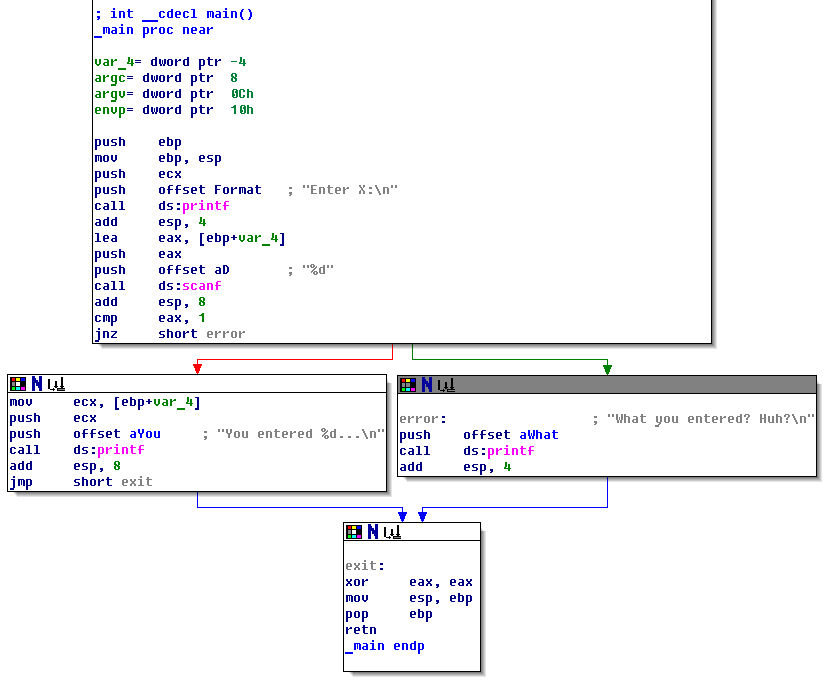
\includegraphics[scale=\FigScale]{patterns/04_scanf/3_checking_retval/IDA.png}
\caption{\RU{Отображение в IDA в виде графа}\EN{Graph mode in IDA}}
\label{fig:ex3_IDA_1}
\end{figure}

\RU{После каждого условного перехода видны две стрелки: зеленая и красная}\EN{There are two arrows
after each conditional jump: green and red}.
\RU{Зеленая ведет к тому блоку, который исполнится если переход сработал, а красная --- если не сработал}
\EN{Green arrow pointing to the block which will be executed if jump is triggered, and red if otherwise}.

\clearpage
\RU{В этом режиме также можно сворачивать узлы и давать им названия}
\EN{It is possible to fold nodes is this mode and give them names as well} (``group nodes'').
\RU{Я сделал это для трех блоков}\EN{I did it for 3 blocks}:

\begin{figure}[H]
\centering
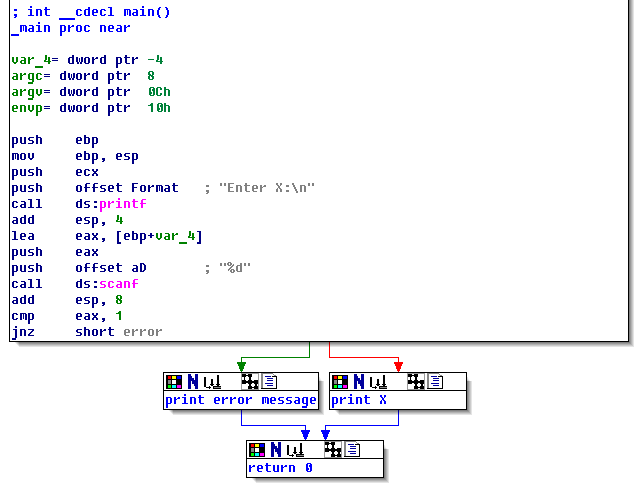
\includegraphics[scale=\FigScale]{patterns/04_scanf/3_checking_retval/IDA2.png}
\caption{\RU{Отображение в IDA в виде графа с тремя свернутыми блоками}\EN{Graph mode in IDA with 3 nodes folded}}
\label{fig:ex3_IDA_2}
\end{figure}

\RU{Всё это очень полезно делать}\EN{It's very useful}.
\RU{Вообще, очень важная часть работы реверсера состоит в том, чтобы уменьшать количество имеющейся информации}
\EN{It can be said, a very important part of reverse engineer's job is to reduce information he/she have}.
\fi

\ifdefined\IncludeOlly
\clearpage
\subsection{MSVC: x86 + \olly}

\RU{Попробуем в \olly немного хакнуть программу, и сделать вид что \scanf срабатывает всегда без ошибок}
\EN{Let's try to hack our program in \olly, forcing it to think \scanf working always without error}.

\RU{Когда в \scanf передается адрес локальной перемейнной, изначальное, в данном случае, 
у нас в этой переменной
находится некий мусор, а это}\EN{When address of local variable is passed into \scanf,
initially this variable contain some random garbage, that is} \TT{0x4CD478}\EN{ in case}:

\begin{figure}[H]
\centering
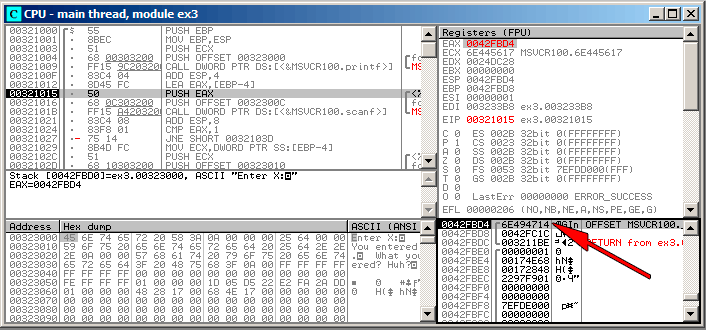
\includegraphics[scale=\FigScale]{patterns/04_scanf/3_checking_retval/olly_1.png}
\caption{\olly: \RU{передача адреса переменной в}\EN{passing variable address into} \scanf}
\label{fig:scanf_ex3_olly_1}
\end{figure}

\clearpage
\RU{Когда}\EN{When} \scanf \RU{запускается, я ввожу в консоли что-то непохожее на число, например}
\EN{is executing, I entered something definitely not a number in the console, like} ``asdasd''.
\scanf \RU{заканчивается с 0 в}\EN{finishing with 0 in} \EAX, \RU{что означает, что произошла ошибка}
\EN{which mean, an error occurred}:

\begin{figure}[H]
\centering
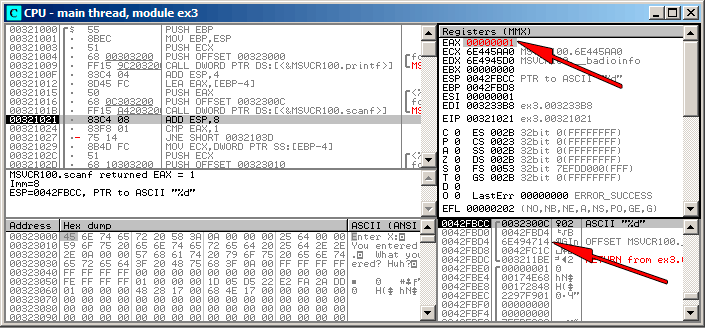
\includegraphics[scale=\FigScale]{patterns/04_scanf/3_checking_retval/olly_2.png}
\caption{\olly: \scanf \RU{закончился с ошибкой}\EN{returning error}}
\label{fig:scanf_ex3_olly_2}
\end{figure}

\RU{Вместе с этим, мы можем посмотреть на локальную переменную в стеке, она не изменилась}
\EN{We can also see to the local variable in the stack and notice that it's not changed}.
\RU{Действительно, ведь что туда записала бы ф-ция \scanf}\EN{Indeed, what \scanf would write there}?
\RU{Она просто ничего не делала кроме возвращения нуля}\EN{It just did nothing except returning zero}.

\clearpage
\RU{Теперь попробуем немного ``хакнуть'' нашу программу}\EN{Now let's try to ``hack'' our program}.
\RU{Кликнем правой кнопкой на}\EN{Let's right-click on} \EAX, \RU{там, в числе опций, будет также}
\EN{there will also be} ``Set to 1''\EN{ among other options}.
\RU{Это то что нам нужно}\EN{This is what we need}.

\RU{В \EAX теперь 1, последующая проверка пройдет как надо, и \printf выведет значение переменной
из стека}\EN{1 now in \EAX, so the following check will executed as we need, and \printf will print
value of variable in the stack}.

\RU{Запускаем}\EN{Let's run} (F9) \RU{и видим в консоли следующее}\EN{and we will see this in 
console window}:

\begin{figure}[H]
\centering
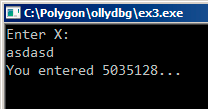
\includegraphics[scale=\FigScale]{patterns/04_scanf/3_checking_retval/olly_3.png}
\caption{\RU{консоль}\EN{console window}}
\end{figure}

\RU{Действительно}\EN{Indeed}, $5035128$ \RU{это десятичное представление числа в стеке}
\EN{is a decimal representation of the number in stack} (\TT{0x4CD478})!

\clearpage
\subsection{MSVC: x86 + Hiew}
\index{Hiew}

\RU{Это еще и может быть простым примером патчинга исполняемого файла}\EN{This can be 
also a simple example of executable file patching}.
\RU{Мы можем попробовать пропатчить его таким образом, что программа всегда будет выводить числа,
вне зависимости от того, что мы вводим}\EN{We may try to patch executable, so the program will always 
print numbers, no matter what we entered}.

\RU{Учитывая, что исполняемый файл скомпилирован с учетом импортирования ф-ций из}\EN{Assuming the 
executable compiled against external} \TT{MSVCR*.DLL} (\RU{т.е., с опцией}\EN{i.e., with} 
\TT{/MD}\EN{ option})\footnote{\RU{то, что еще называют}\EN{that's what also called} ``dynamic linking''}, 
\RU{мы можем отыскать ф-цию}\EN{we may find} \main \RU{в самом начале секции}\EN{function at the 
very beginning of} \TT{.text}\EN{ section}.
\RU{Откроем исполняемый файл в Hiew, найдем самое начало секции}\EN{Let's open executable in Hiew, 
find the very beginning of} \TT{.text}\EN{ section} (Enter, F8, F6, Enter, Enter).

\RU{Мы увидим следующее}\EN{We will see this}:

\begin{figure}[H]
\centering
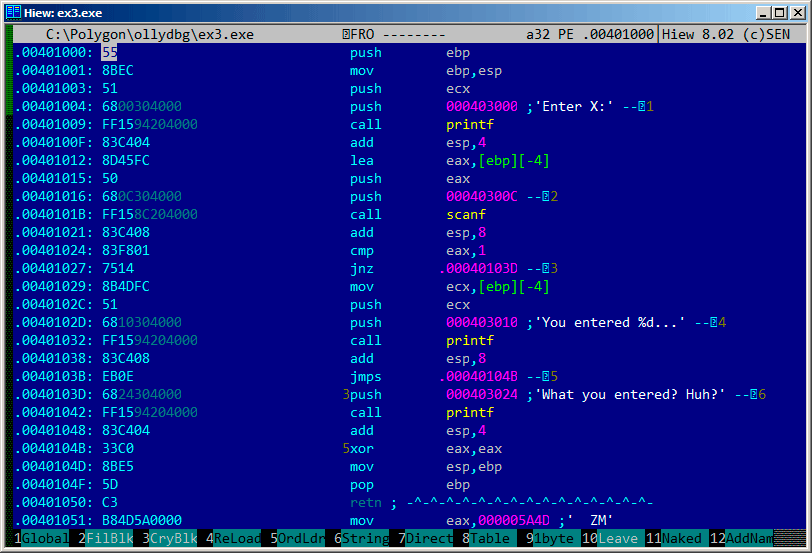
\includegraphics[scale=\FigScale]{patterns/04_scanf/3_checking_retval/hiew_1.png}
\caption{Hiew: \RU{ф-ция }\main\EN{ function}}
\label{fig:scanf_ex3_hiew_1}
\end{figure}

Hiew \RU{находит}\EN{finds} \ac{ASCIIZ}\RU{-строки и показывает их, также как и имена импортируемых 
ф-ций}\EN{ strings and displays them, as well as imported function names}.

\clearpage
\RU{Переведите курсор на адрес}\EN{Move cursor to the address} \TT{.00401027} 
(\RU{с инструкцией}\EN{with the} \TT{JNZ}\RU{, которую мы хотим заблокировать}\EN{ instruction we 
should bypass}), \RU{нажмите}\EN{press} F3,
\RU{затем наберите}\EN{and then type} ``9090'' (\RU{что означает}\EN{meaning two} \ac{NOP}-\RU{а}\EN{s}): 

\begin{figure}[H]
\centering
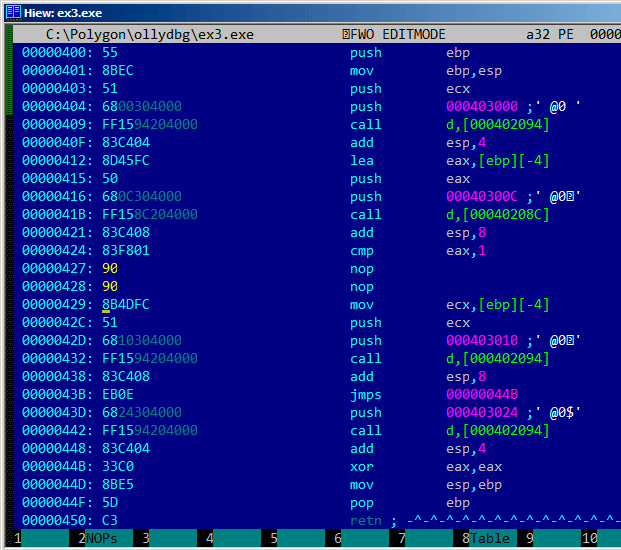
\includegraphics[scale=\FigScale]{patterns/04_scanf/3_checking_retval/hiew_2.png}
\caption{Hiew: \RU{замена}\EN{replacing} \TT{JNZ} \RU{на два}\EN{by two} \ac{NOP}-\RU{а}\EN{s}}
\label{fig:scanf_ex3_hiew_2}
\end{figure}

\RU{Затем}\EN{Then} F9 (update). \RU{Теперь исполняемый файл записан на диск. Он будет вести себя
так, как нам надо.}\EN{Now the executable saved to disk. It will behave as we wanted.}

\RU{Два}\EN{Two} \ac{NOP}-\RU{а}\EN{s} \RU{возможно, не так эстетично, как могло бы быть}\EN{are probably 
not quite \ae{}sthetically as it could be}.
\RU{Другой способ пропатчить инструкцию, это записать 0 во второй байт опкода (смещение перехода),
так что}\EN{Other way to patch this instruction is to write just 0 to the second opcode byte (\gls{jump offset}), 
so that} \TT{JNZ} \RU{всегда будет переходить на следующую инструкцию}\EN{will always jump to 
the next instruction}.

\RU{Можно пропатчить и наоборот: первый байт заменить на \TT{EB}, второй байт (смещение перехода) 
не трогать}
\EN{We can do the opposite: replace first byte to \TT{EB} while not touching the second byte (\gls{jump offset})}.
\RU{Получится всегда срабатывающий безусловный переход}\EN{We'll got here always triggered unconditional
jump}.
\RU{Теперь сообщение об ошибке будет выдаваться всегда, даже если мы ввели число}
\EN{The error message will be printed always, no matter what number was entered}.

\fi

\subsection{MSVC: x64}

\myindex{x86-64}

\ifdefined\RUSSIAN
Так как здесь мы работаем с переменными типа \Tint, а они в x86-64 остались 32-битными, то мы здесь видим, как продолжают использоваться регистры с префиксом \TT{E-}.
Но для работы с указателями, конечно, используются 64-битные части регистров с префиксом \TT{R-}.
\fi

\ifdefined\ENGLISH
Since we work here with \Tint{}-typed variables, which are still 32-bit in x86-64, we see how the 32-bit part of the registers (prefixed with \TT{E-}) are used here as well.
While working with pointers, however, 64-bit register parts are used, prefixed with \TT{R-}.
\fi

\ifdefined\BRAZILIAN
Como trabalhamos aqui com variáveis do tipo \Tint, que ainda são 32-bits no x86-64, nós vemos como a parte de 32-bits dos registradores (com o prefixo \TT{E-}) sao usadas aqui da mesma maneira.
No entanto, quando trabalhamos com ponteiros, as partes dos registradores de 64-bits são usadas, prefixadas com \TT{R-}.
\fi

\lstinputlisting[caption=MSVC 2012 x64]{patterns/04_scanf/3_checking_retval/ex3_MSVC_x64.asm.\LANG}


\ifdefined\IncludeARM
\subsection{ARM}

\subsubsection{ARM: \OptimizingKeilVI (\ThumbMode)}

\lstinputlisting[caption=\OptimizingKeilVI (\ThumbMode)]{patterns/04_scanf/3_checking_retval/ex3_ARM_Keil_thumb_O3.asm}

\index{ARM!\Instructions!CMP}
\index{ARM!\Instructions!BEQ}
\RU{Новые инструкции здесь для нас: \CMP и \ac{BEQ}.}
\EN{New instructions here are \CMP and \ac{BEQ}.}

\CMP \RU{аналогична той что в x86, она отнимает один аргумент от второго и сохраняет флаги.}
\EN{is akin to the x86 instruction bearing the same name, it subtracts one argument from another and saves flags.}
% TODO: в мануале ARM $op1 + NOT(op2) + 1$ вместо вычитания

\index{ARM!\Registers!Z}
\index{x86!\Instructions!JZ}
\ac{BEQ} \RU{совершает переход по другому адресу, 
если операнды при сравнении были равны, 
либо если результат последнего вычисления был $0$, либо если флаг Z равен $1$.}
\EN{is jumping to another address if operands while comparing were equal to each other, or,
if result of last computation was $0$, or if Z flag is $1$.}
\RU{То же что и \JZ в}\EN{Same thing as \JZ in} x86.

\RU{Всё остальное просто: исполнение разветвляется на две ветки, затем они сходятся там, 
где в \Reg{0} записывается $0$ как возвращаемое из функции значение и происходит выход из функции.}
\EN{Everything else is simple: execution flow is forking into two branches, then the branches are 
converging at the point
where $0$ is written into the \Reg{0}, as a value returned from the function, and then function finishing.}

\subsubsection{ARM64}

\lstinputlisting[caption=\NonOptimizing GCC 4.9.1 ARM64,numbers=left]{patterns/04_scanf/3_checking_retval/ARM64_GCC491_O0.s}

\index{ARM!\Instructions!CMP}
\index{ARM!\Instructions!Bcc}
\EN{Code flow is divided here using CMP/BNE (Branch if Not Equal) instructions pair.}
\RU{Исполнение здесь разветвляется используя пару инструкций CMP/BNE (Branch if Not Equal: переход если не равно).}

\fi


\section{\Exercises}

\subsection{\Exercise \#1}
\label{exercise_scanf_1}

\EN{This code, compiled in Linux x86-64 using GCC is crashing while execution (segmentation fault).
However, it works in Windows environment compiled by MSVC 2010 x86.
Why?}
\RU{Этот код, когда компилируется при помощи GCC в Linux x86-64, падает во время исполнения (segmentation fault).
Но он работает в среде Windows, когда скомпилирован при помощи MSVC 2010 x86.
Почему?}

\begin{lstlisting}
#include <string.h>
#include <stdio.h>

void alter_string(char *s)
{
        strcpy (s, "Goodbye!");
        printf ("Result: %s\n", s);
};

int main()
{
        alter_string ("Hello, world!\n");
};
\end{lstlisting}


\Answer{}: \myref{exercise_solutions_scanf_1}.

